\chapter{Preprocesamiento y características}
\section{Preprocesamiento}\label{sec:pre}
El preprocesamiento de datos es una fase crítica que implica la limpieza,
transformación y preparación de los datos, en este caso previo a la aplicación
de técnicas de detección de anomalías, de manera que se puedan analizar, tratar
o modelar de forma efectiva y correcta.

\nocite{herrera2004pre}
\subsection{¿Por qué es necesario?}
Los datos que se obtienen de las fuentes de información suelen estar incompletos,
contener errores o no ser adecuados para el problema que se quiere resolver.
Por ello, es necesario realizar una serie de operaciones sobre los mismos para
poder utilizarlos de forma efectiva.

Además, la preparación del conjunto puede resultar en una reducción de la cantidad
de datos a procesar, lo que puede suponer una mejora en la eficiencia del proceso
a nivel global, uno de los problemas vistos en el capítulo~\ref{sec:issues}.

\subsection{¿Cómo se hace?}
El preprocesamiento de datos se puede dividir en varias fases~\cite{zhang2003data}:

\begin{itemize}[topsep=0pt]
	\item \textbf{Colección e integración:} se obtiene los datos de las diferentes fuentes, se
		resuelven problemas de representación y codificación y se integran los datos para crear
		información homogénea en forma de un solo conjunto.~\cite{detours2003integration}
	\item \textbf{Limpieza:} se resuelven conflictos entre los datos y se comprueba la corrección
		de los mismos.~\cite{kim2003taxonomy}
	\item \textbf{Transformación:} se consolida el conjunto de forma apropiada para la posterior
		extracción de información (en nuestro caso, la detección de anomalías). Este proceso puede
		incluir la sumarización de datos y operaciones de agregación.~\cite{lin2002attribute}
	\item \textbf{Reducción:} se seleccionan los datos relevantes para el problema a resolver y se
		eliminan los datos redundantes.~\cite{liu2012feature}
\end{itemize}

\subsection{¿Qué relación tiene con la detección de anomalías?}
El preprocesamiento de datos es una fase esencial para cualquier proceso de minería de datos. En
el caso de la detección de anomalías, es absolutamente necesario realizar un correcto preprocesado
de los datos para poder aplicar las técnicas de detección (ver~\nameref{chap:tecnicas}) de forma
efectiva.~\cite{ramirez2022cleaning}

\noindent
\begin{minipage}{\linewidth}
	\centering
	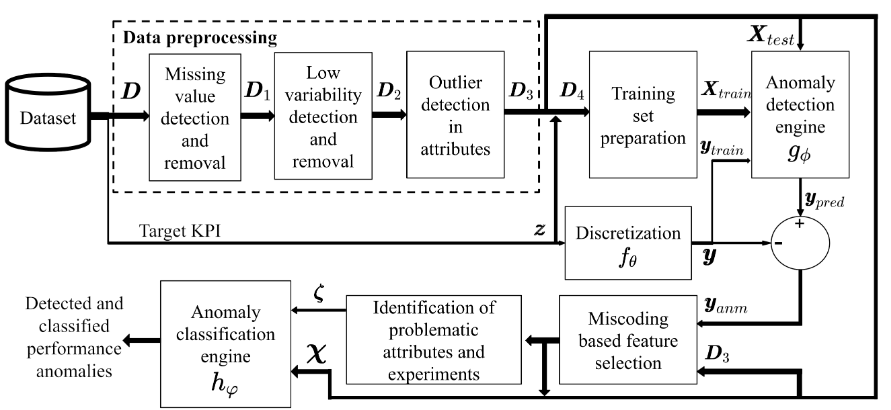
\includegraphics[width=\textwidth]{pre.png}
	\captionof{figure}{Ejemplo de diagrama de flujo de preprocesamiento con detección de
		anomalías (\textit{KLNX})~\cite{ramirez2022cleaning}}\label{fig:fig3}
\end{minipage}

Gracias al modelo resultante de la minería de anomalías, se puede mejorar el preprocesamiento de
conjuntos futuros al descartar outliers durante la fase de limpieza, por lo que se mejora
retroactivamente la calidad de los datos.

\section{Selección de características}\label{sec:feat}
La selección de características~\cite{guyon2003introduction} se enfoca en identificar las variables más relevantes para el
proceso de detección de anomalías. Los puntos clave de esta fase son la siguiente:

\begin{itemize}
	\item \textbf{Relevancia:} se evalúa la importancia de cada característica en
		función de su contribución a la predicción del modelo.
	\item \textbf{Reducción de dimensionalidad:} se reduce el número de características
		eliminando las redundantes o irrelevantes. Una de las técnicas más populares es
		PCA~\cite{wold1987principal} (\textit{Análisis de Componentes Principales}), que
		consiste en la transformación de un conjunto de variables correlacionadas en un
		conjunto de variables no correlacionadas llamadas componentes principales.
	\item \textbf{Técnicas de selección:} se seleccionan las características mediante
		técnicas como \textbf{filters}, \textbf{wrappers} o \textbf{embedded methods},
		cada una con sus características y ventajas.
\end{itemize}

La \textit{feature selection} va mucho más allá que estos puntos y cuenta con una larga lista de
características y tópicos a tener en cuenta (\textit{\textbf{sensiblidad a desequilibrios, validación
y evaluación, interpretación\ldots}}) que no se tratarán en este trabajo, pues es untema muy
amplio digno de un trabajo propio, junto con el preprocesamiento. Pese a esto, ambas fases son
cruciales en cualquier proceso de minería de datos y, por tanto, también en la detección de anomalías.
